\section{Перша робота по оцифровуванню дошки}
У 2004 році інженери з Microsoft Research Zhengyou Zhang
та Li-wei He представили свій алгоритм по скануванню написів
білої дошки \cite{zhang:2004}. Система оброблює фотографії білої дошки, локалізує область
написів, вирівнює у прямокутну форму дошку та бінаризує написи без втрати
кольору (Рис. \ref{fig:zhang:2004}).
\begin{figure}[H]
  \centering
  \subfloat[До обробки]{
      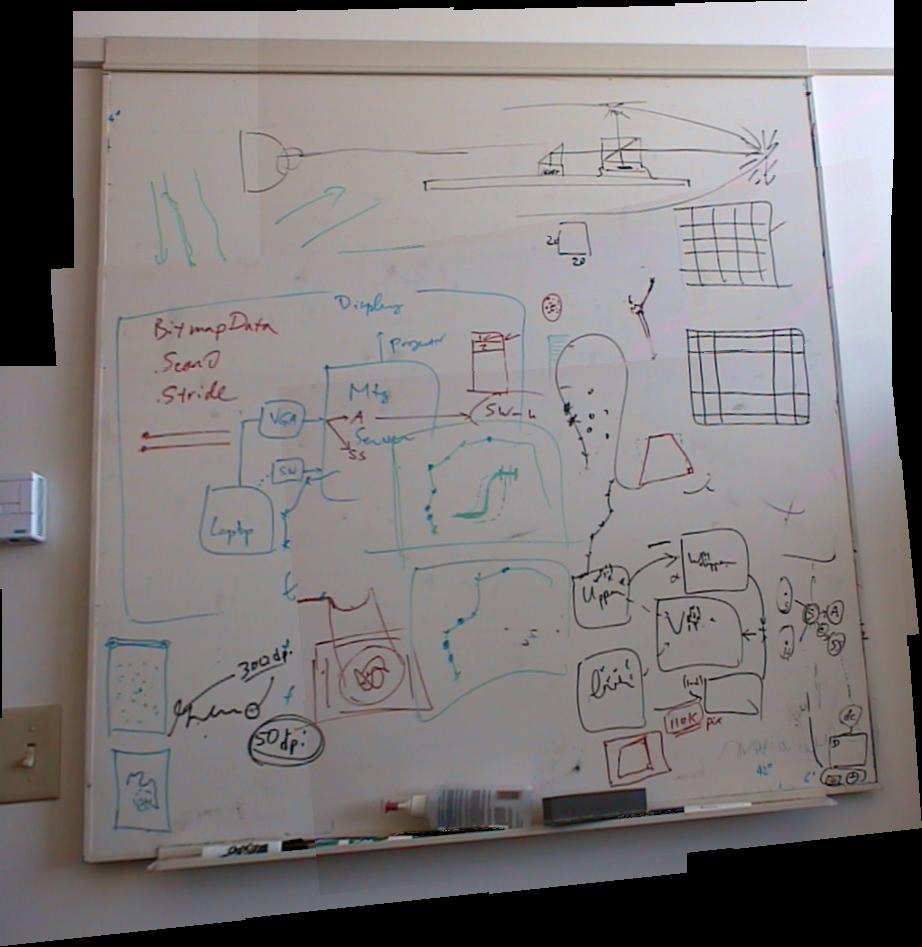
\includegraphics[width=0.4\textwidth]{images/zhang_2004_1}
  }
  \subfloat[Після обробки]{
      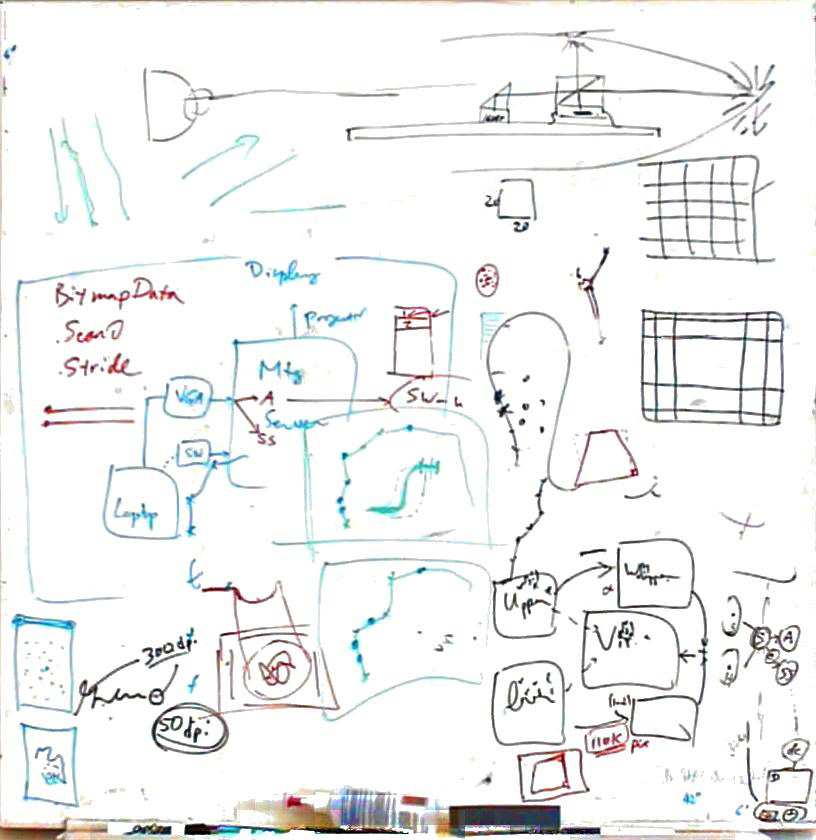
\includegraphics[width=0.4\textwidth]{images/zhang_2004_2}
  }
  \caption{Демонстрація роботи алгоритму інженерів з Microsoft \cite{zhang:2004}
    \label{fig:zhang:2004}
  }
\end{figure}
Також автори реалізували склейку зображень дошки зроблених з різних
ракурсів за допомогою гомографії. Гарна якість оцифрування дошки
досягається насамперед тим, що вона має білий колір, що в свою чергу
накладає обмеження на використання технології з дошками відмінного
від білого кольорів.
У наступній свої роботі \cite{zhang:2007} ці ж самі автори побудували
технологію, яка в реальному часі оброблює відеозапис, видаляє людину біля
дошки за допомогою часової медіани, але тут немає
панорамного склеювання знімків. Головна ідея роботи полягала у розробці
програми для телеконференсій.

\section{Автоматичне сканування дошки}
Автори роботи \cite{wienecke} створили програму яка переводить написи на білій
дошці у цифрові (Рис. \ref{fig:wienecke}). Вони реалізували локалізацію тексту та подальшу
його обробку. Дана технологія не вирішує проблему перекривання викладачем написів
або дошку іншого кольору, відмінного від білого.
\begin{figure}[H]
  \centering
  \subfloat[Детекція написів]{
      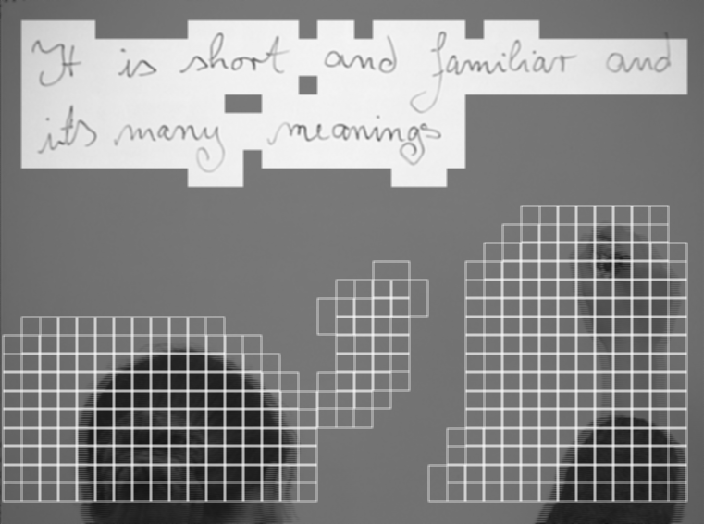
\includegraphics[width=0.4\textwidth]{images/wienecke_1}
  }
  \subfloat[Обробка написів]{
      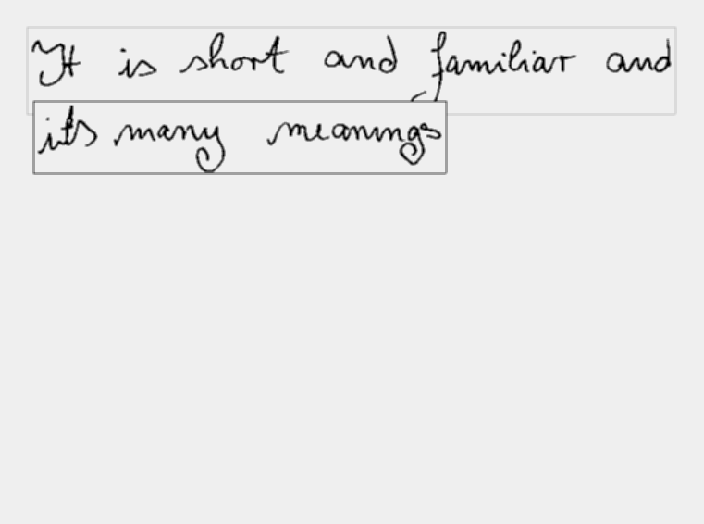
\includegraphics[width=0.4\textwidth]{images/wienecke_2}
  }
  \caption{Демонстрація роботи сканування дошки \cite{wienecke}
    \label{fig:wienecke}
  }
\end{figure}
Можна помітити, що, як і в попередній роботі, гарна якість виокремлення написів
досягається тим що дошка білого кольору.

\section{Відстежування об'єкту та віднімання фону}
У 2012 році науковці зі Стенфордського університету Alex Gonzalez,
Bongsoo Suh, Eun Soo Choi представили технологію \cite{suh} локалізації дошки
(навіть такої, яка розділена на частини), відстеження викладача та його
подальше прибирання. Алгоритм також може працювати з різними кольорами
дошок. Для прибирання викладача і всіх рухомих об'єктів автори також
використали тимчасову медіану (Рис. \ref{fig:suh}).

Дана програма не працює в реальному часі, оскільки всі операції над кадрами
відео займають тривалий час, а також саме відео перед обробкою
піддають компресії.
\begin{figure}[H]
  \centering
  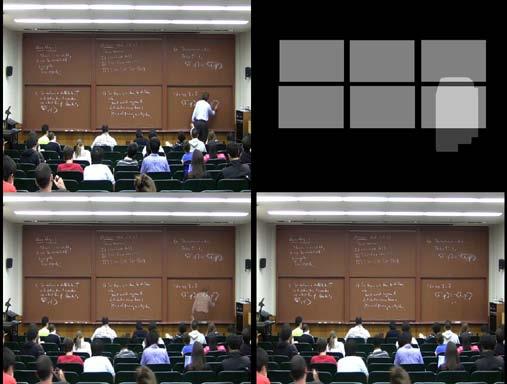
\includegraphics[width=0.6\textwidth]{images/suh}
  \caption{Демонстрація роботи авторів зі Стенфордського університету \cite{suh}
    \label{fig:suh}
  }
\end{figure}
Головною особливістю даної роботи є те, що  алгоритм автоматично локалізує
різну кількість дошок. Однак, варто відмітити, що тестування відбувалось на
відео лекціях де камера знімає всю дошку і не рухається за викладачем.

\section{Відокремлення написів дошки}
У 2014 році науковці із Тайванського університету представили свій аналог \cite{yeh}
алгоритму по оцифровуванні дошки (Рис. \ref{fig:yeh}). Для видалення викладача автори застосували
алгоритм кластеризації k-means. Для отримання бінаризованих написів з дошки
використане адаптивне вирівнювання. Варто відмітити гарну
якість власного методу зменшення шуму.
\begin{figure}[H]
  \centering
  \subfloat[До обробки]{
      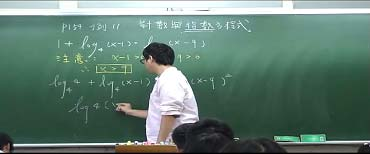
\includegraphics[width=0.6\textwidth]{images/yeh_1}
  }\\
  \subfloat[Після обробки]{
      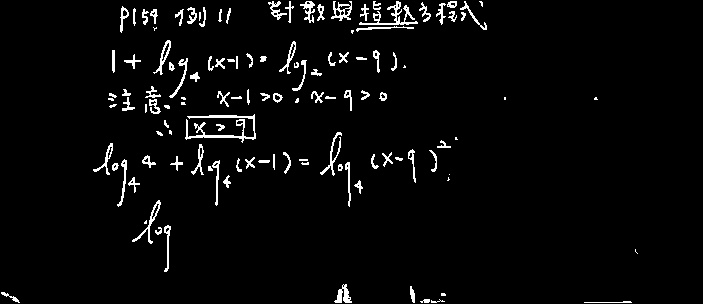
\includegraphics[width=0.6\textwidth]{images/yeh_2}
  }
  \caption{Демонстрація роботи сканування дошки \cite{yeh}
    \label{fig:yeh}
  }
\end{figure}
Автори не надали час обробки всього відео. Щоб отримати якісну сегментацію
дошки та викладача потрібно, щоб кадр містив не тільки викладача, причому одяг викладача
має бути сильно відмінним від кольору дошки. Це потрібно для коректної роботи алгоритму K-means.
Тобто нема гарантії, що якийсь рухомий об'єкт не буде класифікований як дошка під час класифікації.

\section{Сучасна робота}
На даний момент найсучаснішою повноцінною технологією \cite{davila:2017}, яка оцифровує дошку є робота
науковців з університету Рочестер. Автори Kenny Davila та Richard Zanibbi
використали просторово-часовий індекс для виокремлення написів і викладача (Рис. \ref{fig:davila:2017}).
Відбувається видалення не самого викладача,  а його контурів після бінаризації картинки.
Варто відмітити, що і тут камера має бути нерухомою.
\begin{figure}[H]
  \centering
  \subfloat[До обробки]{
      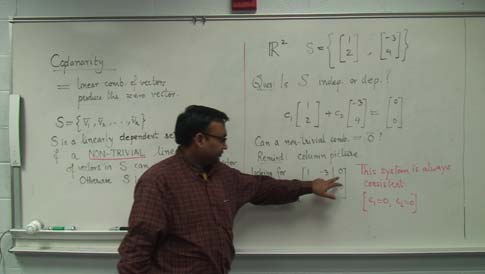
\includegraphics[width=0.6\textwidth]{images/davila_2017_1}
  }\\
  \subfloat[Після обробки]{
      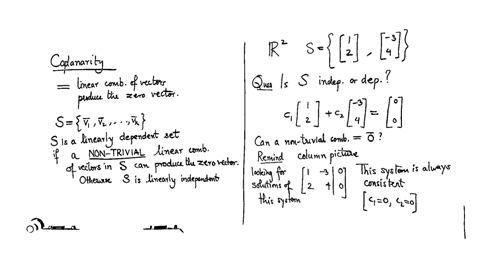
\includegraphics[width=0.6\textwidth]{images/davila_2017_2}
  }
  \caption{Демонстрація роботи сканування дошки \cite{davila:2017}
    \label{fig:davila:2017}
  }
\end{figure}
Пізніше ці ж автори створили повністю згорткову нейронну мережу \cite{davila:2021}
для обробки написів дошки. Дана нейронна мережа LectureNet досить добре бінаризує написи з дошки.
\begin{figure}[H]
  \centering
  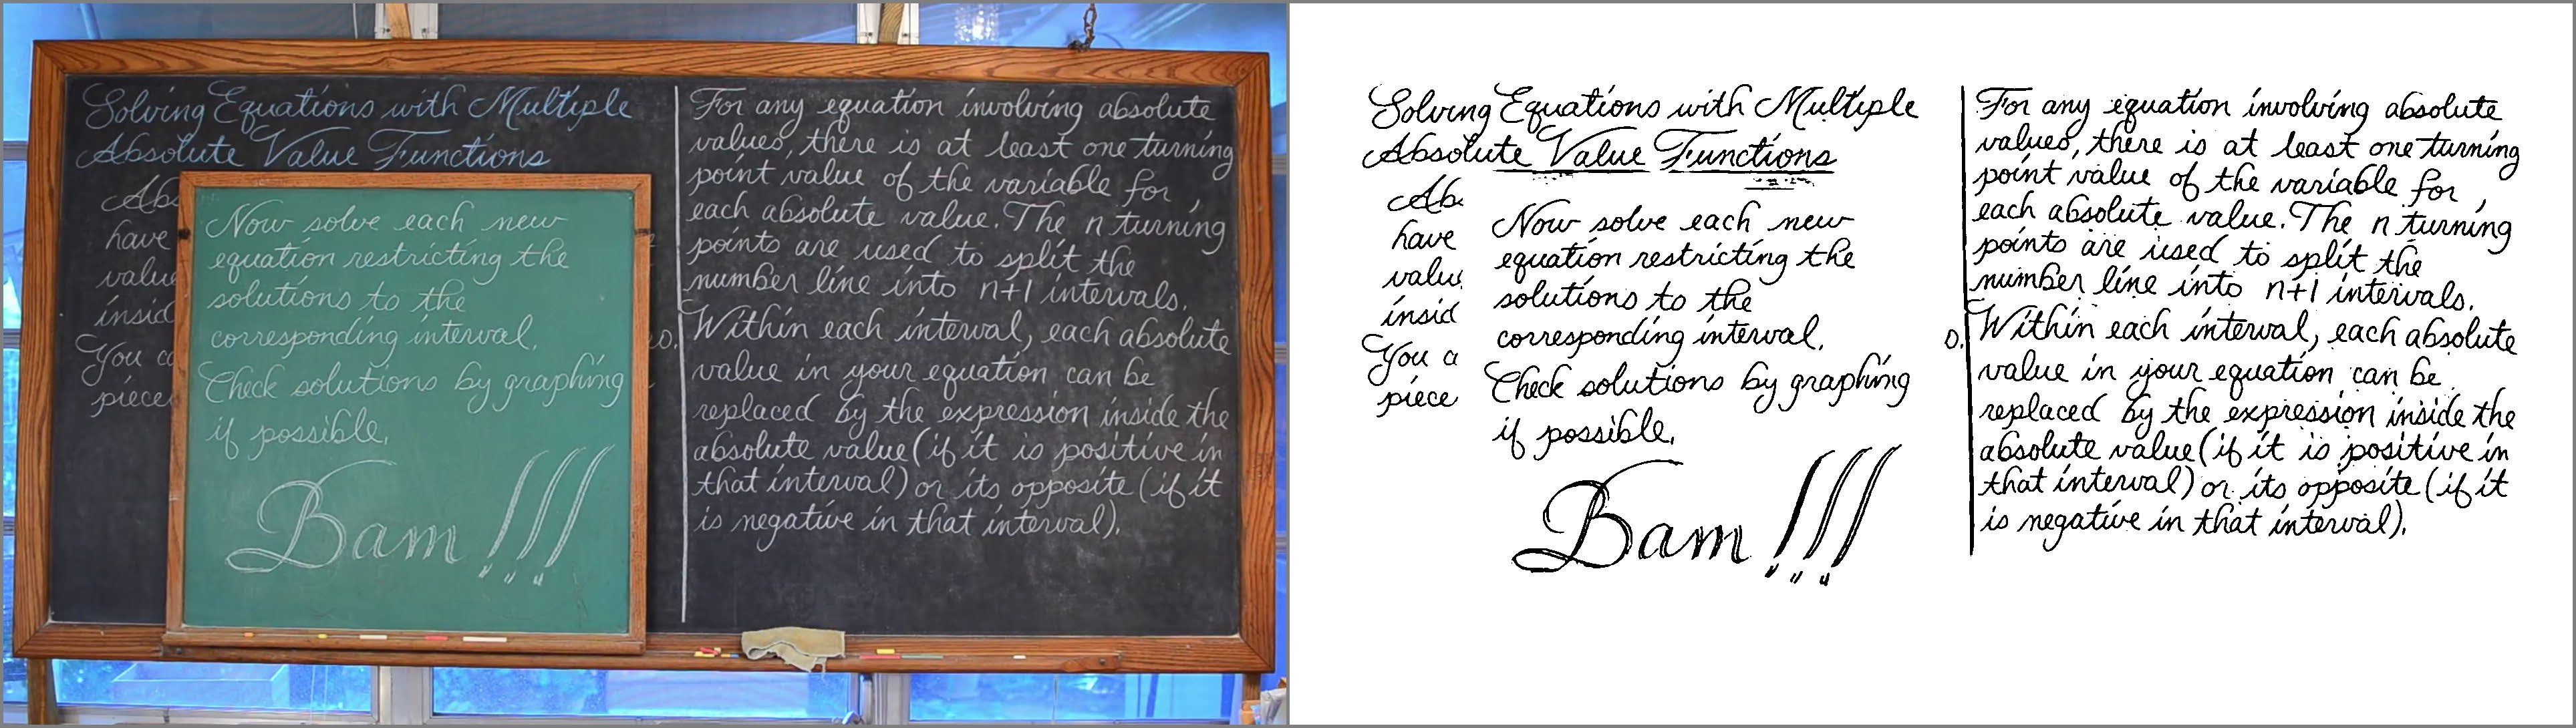
\includegraphics[width=0.8\textwidth]{images/davila_2021}
  \caption{Приклад роботи авторів з Рочестер}
  \label{fig:davila:2021}
\end{figure}

\clearpage